% Goal: 10-minute talk on the informal review "The State of Valuing Urban Ecosystem Services"
% Follows outline.md and manuscript/main.tex section by section. Preamble copied from the ASU JMP deck
% (PhD Work/green_space_spending/presentations/16_ASU/creel_heat_green_spend.tex).
% Andie Creel / Started November 2026

\documentclass[aspectratio=169]{beamer}
\usetheme{Madrid}
\usepackage{bookmark}

% Include graphicx package for images
\usepackage{graphicx}
\usepackage{lmodern}
\usepackage{tikz}
\usetikzlibrary{arrows.meta, decorations.pathreplacing}
\usepackage{adjustbox}

% tables
\usepackage{booktabs}
\usepackage{array}
\usepackage{colortbl} % \rowcolor for shaded table rows

% citations
\usepackage{xcolor}
\usepackage[authoryear]{natbib}
\bibpunct{%
    \textcolor{gray}{(}}{%    opening delimiter
    \textcolor{gray}{)}}{%    closing delimiter
  \textcolor{gray}{;}}{a}{,}{,}%        separator (gray to match citecolor), mode=a (author–year), punctuation
\usepackage{hyperref}    % <– actually load hyperref
\hypersetup{
  colorlinks   = true,
  linkcolor    = white,  % internal slide links
  citecolor    = gray,   % author–year citations (text + gray parens)
  urlcolor     = blue
}
% hyperref (2026) leaves natbib's author-year break as a no-op in beamer, which drops the ", " between author and year
% (restored here, in gray to match citecolor)
\makeatletter
\AtBeginDocument{\def\hyper@natlinkbreak#1#2{\hyper@linkend\textcolor{gray}{#1}\hyper@linkstart{cite}{cite.#2}}}
\makeatother
\newcommand{\smallcite}[1]{\begingroup\scriptsize\citep{#1}\endgroup}
\newcommand{\gt}{>}


% Remove colored box from slide headers (frametitle)
\setbeamertemplate{frametitle}{%
    \vskip1ex
    \color{black}\insertframetitle%
    \vskip1ex
}

% set block colors
\setbeamercolor{block title}{bg=gray!40, fg=black}
\setbeamercolor{block body}{bg=gray!10, fg=black}


% Change footer colors to a more aesthetically pleasing black, white, and gray theme
\setbeamercolor{author in head/foot}{bg=black, fg=white}
\setbeamercolor{title in head/foot}{bg=darkgray, fg=white}
\setbeamercolor{date in head/foot}{bg=black, fg=white}
\setbeamertemplate{itemize items}{-}
\setbeamercolor{itemize item}{fg=black}
\setbeamercolor{itemize subitem}{fg=black}
\setbeamercolor{enumerate item}{fg=black}
\setbeamercolor{enumerate subitem}{fg=black}

% Customizing the footer
\setbeamertemplate{footline}
{
    \leavevmode%
    \hbox{%
    \begin{beamercolorbox}[wd=.3\paperwidth,ht=2.5ex,dp=1ex,left]{author in head/foot}%
        \hspace*{1em}\usebeamerfont{author in head/foot}\insertshortauthor
    \end{beamercolorbox}%
    \begin{beamercolorbox}[wd=.4\paperwidth,ht=2.5ex,dp=1ex,center]{title in head/foot}%
        \usebeamerfont{title in head/foot}\insertshorttitle
    \end{beamercolorbox}%
    \begin{beamercolorbox}[wd=.3\paperwidth,ht=2.5ex,dp=1ex,right]{date in head/foot}%
        \hspace*{1em}\insertframenumber
        \hspace*{1em}\usebeamerfont{date in head/foot}\insertshortdate\hspace*{1em}
    \end{beamercolorbox}}%
    \vskip0pt%
}

% Remove navigational buttons:
\setbeamertemplate{navigation symbols}{}


% Redefine the title page to remove boxes and set the title color to black
\setbeamertemplate{title page}{
  \vbox{}
  \vfill
\begin{center}
        {\usebeamerfont{title}\color{black}\inserttitle\par}
        \vskip1em
        {\usebeamerfont{author}\insertauthor\par}
        \vskip0.5em
        {\usebeamerfont{date}\insertdate\par}
        \vskip0.5em
        {\usebeamerfont{institute}\insertinstitute\par}
\end{center}
  \vfill
}

% Information to be included in the title page
\title[Valuing Urban Ecosystem Services]{The State of Valuing Urban Ecosystem Services}
%\subtitle{}
\author[Andie M. Creel]{Andie M. Creel}
\date[November 2026]{November 9 2026} 
\institute{Urban Ecosystem Services Workshop - Yale/Gund/NatCap } 

\begin{document}

% --------- Title Page -----------
\usebackgroundtemplate{
    \tikz\node[opacity=0.4] {
        \includegraphics[width=\paperwidth,height=\paperheight]{photos/new_haven_sun_trees.jpg}
    };
}

\begin{frame}
    \titlepage
\end{frame}


% --------- Motivation -----------
\usebackgroundtemplate{}

\begin{frame}{Lay of the Land}
    \begin{itemize}
        \item Urban natural assets (parks, street trees, wetlands, rivers) provide heat control, cleaner air and water, flood mitigation, a place to recreate, and better physical and mental health \smallcite{keelerSocialecologicalTechnologicalFactors2019,baro_mapping_2016}
        \pause \item A large and growing literature  \smallcite{veerkampReviewStudiesAssessing2021,maReviewMethodsQuantifying2025, maReviewMethodsQuantifying2025}:
        \begin{itemize}
            \item Most studied: local temperature regulation (36\% of studies) and recreation (23\%) \smallcite{veerkampReviewStudiesAssessing2021}
            \item Large, publicly owned natural assets (\textit{e.g.,} parks) are studied most often
            \item Still gaps: Value of benefits (especially private benefits), and smaller or less visible natural assets
        \end{itemize}
        \pause \item Despite size of literature, it is hard to translate this literature into decisions about urban nature
    \end{itemize}
\end{frame}

% --------- Challenges -----------

\begin{frame}{Challenges}
    \begin{itemize}
        \item \textbf{No shared definition:} Half of $>$300 reviewed papers never define ``ecosystem service'' \smallcite{tanConceptualFrameworkUntangle2020}
        \begin{itemize}
            \item Definitions vary across fields, and within them \smallcite{boydWhatAreEcosystem2007}
        \end{itemize}
        \pause \item \textbf{No shared method:} At least 47 methods for quantifying urban ecosystem services \smallcite{maReviewMethodsQuantifying2025}
        \pause \item \textbf{Benefits are rarely measured:} 59\% of papers quantify ecosystem functions/properties, a minority state the benefit to people, even fewer in dollars \smallcite{veerkampReviewStudiesAssessing2021}
        \pause \item \textbf{\textit{Why dollars matter:}} \\
        (spoiler, it's not to sell ecosystem services to highest bidder)
        \begin{itemize}
            \item A city needs to know value of ecosystem services for benefit-cost analysis \\
            (trees vs. schools, roads, safety)
            \item Quantifying private benefit (increased revenue, cost savings) can mobilize private money 
            \item A non-profit can use valuation studies to tell funders what a dollar spent on nature returns
        \end{itemize}
    \end{itemize}
\end{frame}

% --------- What is an ecosystem service? -----------

\begin{frame}{Consensus is hard to build when you talk past each other}

    \begin{itemize}
        \item Each of these three papers are cited 2,700--4,200 times on Google Scholar
        \item Flood prevention is a service in one paper and a benefit in another
    \end{itemize}


    \vspace{.7cm}
    \small
    \centering
    {\hypersetup{citecolor=black} % black column titles in this table only
    \renewcommand{\arraystretch}{1.3}
    \begin{tabular}{>{\raggedright\arraybackslash}p{.19\textwidth} >{\raggedright\arraybackslash}p{.23\textwidth} >{\raggedright\arraybackslash}p{.23\textwidth} >{\raggedright\arraybackslash}p{.23\textwidth}}
        \toprule
         & \citeauthor{haines-youngLinksBiodiversityEcosystem2010} (\citeyear{haines-youngLinksBiodiversityEcosystem2010}) & \citeauthor{gomez-baggethunClassifyingValuingEcosystem2013} (\citeyear{gomez-baggethunClassifyingValuingEcosystem2013}) & \citeauthor{boydWhatAreEcosystem2007} (\citeyear{boydWhatAreEcosystem2007}) \\
        \midrule
        \rowcolor{gray!15}
        Wetland & Ecosystem (structure) & & Service \\
        Water slowing or soaking into soil & Function and a service & Function & Input to services \\
        \rowcolor{gray!15}
        Flood control & Justification for why the function counts as a service & Service & Benefit \\
        \bottomrule
    \end{tabular}
    }
    \raggedright

\end{frame}

% three key terms (diagram from manuscript Figure 1)
\begin{frame}{We Want To Communicate! -- Three Key Concepts}
    \centering
    \begin{adjustbox}{max width=.8\textwidth, max totalheight=.52\textheight}
    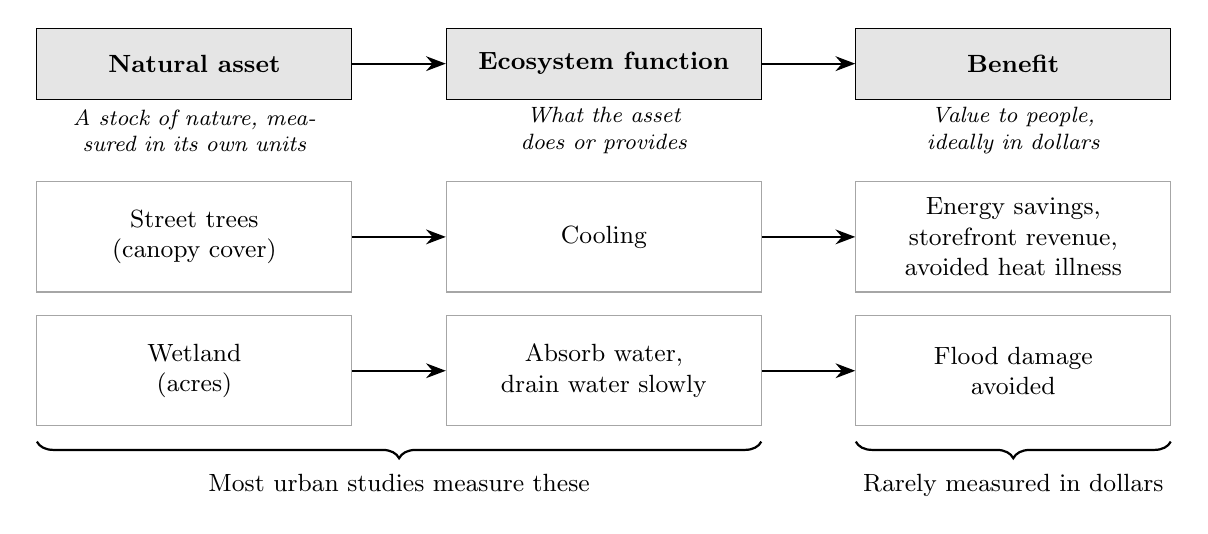
\begin{tikzpicture}[
      font=\small,
      head/.style={draw, fill=gray!20, minimum width=4cm, minimum height=0.9cm, align=center, font=\small\bfseries},
      def/.style={text width=4cm, align=center, font=\footnotesize\itshape},
      ex/.style={draw=gray!70, minimum width=4cm, minimum height=1.4cm, align=center},
      arr/.style={-{Stealth[length=2.5mm]}, thick}
    ]
      % Column headers and definitions
      \node[head] (a) at (0,0)    {Natural asset};
      \node[head] (s) at (5.2,0)  {Ecosystem function};
      \node[head] (b) at (10.4,0) {Benefit};
      \draw[arr] (a) -- (s);
      \draw[arr] (s) -- (b);
      \node[def] at (0,-0.85)    {A stock of nature, measured in its own units};
      \node[def] at (5.2,-0.85)  {What the asset does or provides};
      \node[def] at (10.4,-0.85) {Value to people, ideally in dollars};
      % Example: trees
      \node[ex] (a1) at (0,-2.2)    {Street trees\\(canopy cover)};
      \node[ex] (s1) at (5.2,-2.2)  {Cooling};
      \node[ex] (b1) at (10.4,-2.2) {Energy savings,\\storefront revenue,\\avoided heat illness};
      \draw[arr] (a1) -- (s1);
      \draw[arr] (s1) -- (b1);
      % Example: wetland
      \node[ex] (a2) at (0,-3.9)    {Wetland\\(acres)};
      \node[ex] (s2) at (5.2,-3.9)  {Absorb water, \\drain water slowly};
      \node[ex] (b2) at (10.4,-3.9) {Flood damage\\avoided};
      \draw[arr] (a2) -- (s2);
      \draw[arr] (s2) -- (b2);
      % Where the literature is
      \draw[decorate, decoration={brace, mirror, amplitude=6pt}, thick]
        (-2,-4.8) -- (7.2,-4.8) node[midway, below=8pt] {Most urban studies measure these};
      \draw[decorate, decoration={brace, mirror, amplitude=6pt}, thick]
        (8.4,-4.8) -- (12.4,-4.8) node[midway, below=8pt] {Rarely measured in dollars};
    \end{tikzpicture}
    \end{adjustbox}

    \raggedright
    \small
    \begin{itemize}
        \pause \item Natural capital accounting puts a dollar value on a unit of the asset, but it is technically hard \smallcite{fenichelNewEra2024}
        \item \textbf{Quantifying benefits perfectly should not be the enemy of measuring them at all!}
        \pause \item Cultural and spiritual services (\textit{e.g.,} a river's spiritual value) are important, but hard to price \smallcite{maher_economics_2020,boydWhatAreEcosystem2007}; not my expertise
    \end{itemize}
\end{frame}

% --------- Established functions -----------

% Optional if time: Keeler et al. Table 1 (manuscript Figure 2)
\begin{frame}{Many natural asset's functions are fairly well documented}
    \centering
    \includegraphics[width=\textwidth]{../figures/Keeler_table_1_annotated.png}
    \begin{minipage}{.9\textwidth}
        \raggedright
        \footnotesize Notes: Table 1 of \citet{keelerSocialecologicalTechnologicalFactors2019} in \textit{Nature Sustainability}. Their nature-based solutions are my natural assets; their urban ecosystem services are my ecosystem functions.
    \end{minipage}
\end{frame}

% Optional if time: Keeler et al. Table 1 (manuscript Figure 2)
% \begin{frame}{Value of these assets and their functions is not well understood}
%     \begin{itemize}
%         \item We know these functions exist. 
%         \item What we still need: who benefits, and by how much
%         \item Most studies identify where natural assets are, and what their functions are (59\%); minority state why those functions benefits to people \smallcite{veerkampReviewStudiesAssessing2021}. Fewer still in dollars.
%         \item Simple methods dominate: value transfer ($\approx$47\%) and cost-savings (36\%) \smallcite{maReviewMethodsQuantifying2025}
%         \item Tons of variation in literature: \$5--\$402 per tree per year \smallcite{keelerSocialecologicalTechnologicalFactors2019}
%         \begin{itemize}
%             \item Variation due to different true value across cities, valuation method used, or functions included in the scope of the study. 
%             \item Valuation studies should typically be considered a lower bound on the true value of natural assets.
%         \end{itemize}
        
%     \end{itemize}
% \end{frame}


% Heat mitigation (manuscript Section 3.1)
\begin{frame}{Heat mitigation: the benefit of cooling has been valued in several ways}
    \small
    \begin{itemize}
        \item \textbf{Natural assets:} trees, parks, green roofs, green walls
        \item \textbf{Function:} cooling through shade and evapotranspiration \smallcite{mohajeraniUrbanHeatIsland2017,wongGreeneryMitigationAdaptation2021}
        \begin{itemize}
            \item Greenery lowers peak surface temps 2--9~°C \smallcite{wongGreeneryMitigationAdaptation2021}
            \item Phoenix: vegetation cools the surface by nearly 25~°C vs.\ bare soil \smallcite{jenerette_ecosystem_2011}
        \end{itemize}
        \item \textbf{Benefit:} lower energy bills, steadier business revenue on hot days, increased health
        \item \textbf{What we know in dollars:}
        \begin{itemize}
            \item Phoenix households would pay \$72/month for 1~°F cooler \smallcite{klaiberItLessHot2017}
            \item Trees in major U.S. cities saved \$539M in cooling energy in 2016 \smallcite{herisPilotingUrbanEcosystem2021}
            \item Green space around a business raises revenue 0.5 pct.\ points on days $\geq$100~°F \smallcite{creelValueNatureBasedAdaptation2026}
        \end{itemize}
        \item \textbf{What we don't know:} Value of health benefits of cooling, such as reduced heat-related illness and mortality (more later), private incentive to invest in cooling infrastructure
    \end{itemize}
\end{frame}

% Recreation (manuscript Section 3.4)
\begin{frame}{Recreation: valued in dollars, but how much is due to nature is unclear}
    \small
    \begin{itemize}
        \item \textbf{Natural assets:} parks, trails, water bodies, tree-lined sidewalks
        \item \textbf{Function:} a place to recreate and spend leisure time outside
        \begin{itemize}
            \item Most U.S. outdoor recreation is local: walking, playing with kids or pets \smallcite{creelNationalValueLocal2026}
            \item Poorly understood function: Parks also build social ties among neighbors \smallcite{kazmierczakContributionLocalParks2013,petersSocialInteractionsUrban2010}. Do they increase social cohesion?
        \end{itemize}
        \item \textbf{Benefit:} the value people get from leisure time outside
        \item \textbf{What we know in dollars:}
        \begin{itemize}
            \item Local outdoor recreation: \$5--\$6 per trip, $\approx$\$93B/year \smallcite{creelNationalValueLocal2026}
            \item Lower crime ``unlocked'' $\approx$\$7B in property value near parks \smallcite{albouy_unlocking_2020}
            \item Germans would pay \texteuro 20.25/month for more natural green space \smallcite{bronnmannValueNaturalnessUrban2023}
        \end{itemize}
        \item \textbf{What we don't know:} how much visits are driven by various amenities of a park; the value of social ties
        \begin{itemize}
            \item NYC: fewer social media posts in parks with more green space \smallcite{hamstead_geolocated_2018}
        \end{itemize}
    \end{itemize}
\end{frame}

% Stormwater regulation (manuscript Section 3.2)
\begin{frame}{Stormwater: well studied, but its dollar value leaves out flood damage}
    \small
    \begin{itemize}
        \item \textbf{Natural assets:} trees, parks, wetlands, and other permeable surfaces (rain gardens, swales)
        \item \textbf{Function:} intercept and absorb rainfall, so less runoff \smallcite{veerkampReviewStudiesAssessing2021,herisPilotingUrbanEcosystem2021}
        \begin{itemize}
            \item Unclear how well each assets reduce flooding \smallcite{diepEmpoweringCitiesGlobally2025}; trees work best in small storms \smallcite{herisPilotingUrbanEcosystem2021}
        \end{itemize}
        \item \textbf{Benefit:} less flood damage, lower wastewater treatment costs, fewer sewage overflows
        \item \textbf{What we know in dollars:} limited work
        \begin{itemize}
            \item Trees in major U.S. cities intercepted 2.6B m$^3$ of rain in 2016, worth \$425M \smallcite{herisPilotingUrbanEcosystem2021}
            \item Avoided treatment costs (\$2.58/m$^3$), only in cities with combined sewers
        \end{itemize}
        \item \textbf{What we don't know:} the value of avoided flood damage to homes and businesses
    \end{itemize}
\end{frame}

% Health (manuscript Section 3.5)
\begin{frame}{Health has been valued mainly through avoided heat deaths}
    \small
    \begin{itemize}
        \item \textbf{Natural assets:} parks, trees, and green space more broadly
        \item \textbf{Function:} Many functions contribute to health. Health is a benefit of cooling, cleaner air, and a place for activity, social contact, and rest from stress \smallcite{jenningsApproachingEnvironmentalHealth2015,keelerSocialecologicalTechnologicalFactors2019}
        \item \textbf{Benefit:} fewer heat- and pollution-related deaths and hospital visits; better mood/lower stress
        \begin{itemize}
            \item In less green ZIPs, heat raises odds of elderly cardiovascular death 17\% \smallcite{gronlundVulnerabilityExtremeHeat2015}
            \item Losing 100M ash trees $\rightarrow$ 15,080 more cardiovascular deaths \smallcite{donovanRelationshipTreesHuman2013}
            \item Green space use tied to better well-being \smallcite{jenningsApproachingEnvironmentalHealth2015}
            \item Heat raises mental health helpline calls 3.7\% \smallcite{janzenTemperatureMentalHealth2025}
            \item Mostly observational and confounded by wealth \smallcite{donovanRelationshipTreesHuman2013,ogletreeRelationshipGreenspaceExposure2023}
        \end{itemize}
        \item \textbf{What we know in dollars:} tree cover in 97 U.S. cities avoids $\approx$296 heat deaths/year, worth \$1.0--\$2.4B/year \smallcite{mcdonaldValueUSUrban2020}
        \item \textbf{What we don't know:} How much money insurance companies save from avoided heat-related health damage
    \end{itemize}
\end{frame}

% --------- Distribution -----------

\begin{frame}{Natural assets are unequally distributed}
    \begin{itemize}
        \item Fewer natural assets:
        \begin{itemize}
            \item Historically redlined neighborhoods have less tree canopy \smallcite{locke_residential_2020}
            \item Less affluent neighborhoods have less protected land\smallcite{simsEnvironmentalJusticeCriteria2022}
        \end{itemize}
        \item More heat:
        \begin{itemize}
            \item Historically redlined neighborhoods are hotter \smallcite{hoffmanEffectsHistoricalHousing2020,wilsonUrbanHeatManagement2020,conzelmannLongTermEffectsRedlining2022}
            \item Black residents are more likely than white to live with little tree canopy and mostly impervious surface \smallcite{jesdale_racialethnic_2013}
        \end{itemize}
        \item Benefit valuation across demographics is sensitive to the method used:
        \begin{itemize}
            \item Valuing travel time with a replacement wage instead of 1/3 own wage: richest quintile's value per trip goes from 10$\times$ the poorest's to 1.5$\times$ \smallcite{creelNationalValueLocal2026}
            \item Tree cover where people shop is nearly uncorrelated with customers' income \smallcite{creelValueNatureBasedAdaptation2026}
        \end{itemize}
    \end{itemize}
\end{frame}

% --------- Urban animals -----------

\begin{frame}{Urban animals: the next frontier of ecosystem service measurement?}
    \begin{itemize}
        \item Big gap: function of animals in cities
        \begin{itemize}
            \item Review of 317 papers finds only 2 studies on how animal traits affect an ecosystems' functions \smallcite{schwarzUnderstandingBiodiversityecosystemService2017}
            \item Outside cities: bats and birds control pests $\rightarrow$ big cost savings for farmers \smallcite{frankEconomicImpactsEcosystem2024,noackValueBiodiversityEvidence2025}, wolves cut deer-vehicle collisions, saving $>$\$375K per county per year \smallcite{raynorWolvesMakeRoadways2021}
        \end{itemize}
        \item Possible urban services:
        \begin{itemize}
            \item Coyotes and foxes may keep rats in check $\Rightarrow$ less disease spread \smallcite{boydWhatAreEcosystem2007}
            \item Vultures in India: their collapse raised death rates $>$4\%, more in cities \smallcite{frankSocialCostsKeystone2023}
            \item Birding: a newly recognized bird species is worth $\approx$\$277 per visitor \smallcite{wardleRecreationalValueRare2025}
        \end{itemize}
        \item \textbf{Challenge:} Satellites can see green and blue space, but they cannot do population surveys
        \begin{itemize}
            \item Counting animals takes ground data (\textit{e.g.,} eBird, camera traps) \smallcite{wardleRecreationalValueRare2025,kohlQuantifyingUrbanWildlife2024}
            \item Without data, hard to measure the function of animals in cities, much less their benefit
        \end{itemize}
    \end{itemize}
\end{frame}

% --------- Building natural assets -----------
\usebackgroundtemplate{
    \tikz\node[opacity=0.3] {
        \includegraphics[width=\paperwidth,height=\paperheight]{photos/park-people-nyc.jpg}
    };
}

\begin{frame}
    \begin{center}
        \Huge From Measuring Ecosystem Services\\to Building Natural Assets\\
        \vspace{.5cm}
        \Large Who has the ability, power, and money to make new urban natural assets?
    \end{center}
\end{frame}

\usebackgroundtemplate{}

\begin{frame}{Cities build most new natural assets, often with non-profit partners}
    \begin{itemize}
        \item New natural assets come from restoration, conservation, or (for animals) reintroduction
        \begin{itemize}
            \item Ex: Urban Resources Initiative in New Haven restores abandoned lots into parks and plants trees with communities \smallcite{chenMoreExtremelyHot2024}
        \end{itemize}
        \item Usually the city, often with a non-profit or a business improvement district
        \begin{itemize}
            \item Cities own the land (sidewalks, parks), but have limited budgets and coordination frictions with private actors \smallcite{toxopeusReviewingFinancingBarriers2021}
            \item Private park organizations (mostly non-profits) are $>$40\% of park spending in St. Louis and Detroit \smallcite{tplCityParkFacts2025}
        \end{itemize}
        \item Insurers invest where nature lowers their claims
        \begin{itemize}
            \item 16 Canadian insurers fund wetland restoration to reduce flood risk \smallcite{kouskyNatureInsuranceInsurance2025}
            \item Coral reef insurance in Quintana Roo, Mexico \smallcite{schelskeInsuringNaturalEcosystems2021}
        \end{itemize}
        \item Barriers to more private money: coordinating public and private financiers, and knowing the private benefit \smallcite{toxopeusReviewingFinancingBarriers2021}
    \end{itemize}
\end{frame}

\begin{frame}{Research can unlock financing by measuring who benefits}
    \begin{itemize}
        \item \textbf{Public:} Benefit-cost analysis to win grants or justify municipal budgets
        \begin{itemize}
            \item 2023 revisions to Circulars A-4 and A-94 addressed ecosystem services; rescinded, but still good guidance \smallcite{gilligham_reep,sarinskyLegalDynamicsRescinding2025}
            \item Loss of bats lowers county property tax revenue \$1.2M per year (3.8\%) \smallcite{nakhmurinaFiscalImpactBiodiversity2025}
        \end{itemize}
         \item \textbf{Private:} Identify who benefits, and by how much
        \begin{itemize}
            \item Tree cover protects storefront revenue from heat. In the southern U.S., avoided losses cover the cost of 10\% tree cover in $\approx$4 years (revenue is not profit) \smallcite{creelValueNatureBasedAdaptation2026}
            \item Heat lowers retail consumption \smallcite{leeExtremeTemperaturesAdaptation2025} and labor productivity \smallcite{dasguptaHeatStressLabour2024}, trees lower cooling costs \smallcite{herisPilotingUrbanEcosystem2021,hanCoolCitiesValue2024}
        \end{itemize}
        \item \textbf{Health is an untapped private incentive}
        \begin{itemize}
            \item Health insurers hold a tremendous amount of money; Medicare and Medicaid are among the largest federal budget items
            \item Insurers already invest in natural assets that lower risk \smallcite{kouskyNatureInsuranceInsurance2025,schelskeInsuringNaturalEcosystems2021}
            \item But hospital visits, treatment, and mental health are the benefits we have measured least
        \end{itemize}
    \end{itemize}
\end{frame}

%---- Conclusion  ----
\usebackgroundtemplate{
    \tikz\node[opacity=0.25] {
        \includegraphics[width=\paperwidth,height=\paperheight]{photos/new_haven_sun_trees.jpg}
    };
}

\begin{frame}{Conclusion}
    \begin{itemize}
        \item Large literature, but no shared definition or method, and benefits are rarely measured in dollars
        \item Natural asset $\rightarrow$ ecosystem function $\rightarrow$ benefit
        \item Natural assets' function in cooling, draining stormwater/flood control, providing a place to recreate and supporting health are fairly well established
        \begin{itemize}
            \item What is missing: who benefits, and by how much
        \end{itemize}
        \item Natural assets are unequally distributed across neighborhoods
        \item Urban animals are a gap, partly because we cannot count them from space
        \item Importance
        \begin{itemize}
            \item Measuring public and private benefits can unlock money to build new natural assets $\rightarrow$ health may be the biggest untapped source
        \end{itemize}
    \end{itemize}
\end{frame}

%%%%%%%%%%%%%%%%%%%%%%%%%%%%%%%%%%%%%%%%%%%%%%%%%%%%%%%%%%%%%%%%%%%%%%%%%%%%%
%                           QUESTIONS
%%%%%%%%%%%%%%%%%%%%%%%%%%%%%%%%%%%%%%%%%%%%%%%%%%%%%%%%%%%%%%%%%%%%%%%%%%%%%
\usebackgroundtemplate{
    \tikz\node[opacity=0.7] {
        \includegraphics[width=\paperwidth,height=\paperheight]{photos/green_city.jpg}
    };
}

\begin{frame}
    \begin{center}
        \Huge Questions?\\
        \vspace{1em}
        \normalsize andie.creel@yale.edu
    \end{center}
\end{frame}

% ---- References ----
\usebackgroundtemplate{}


\begin{frame}[allowframebreaks]{References}
    \tiny  % Makes text much smaller; alternatively use \scriptsize or \footnotesize
    \bibliographystyle{abbrvnat}
    \bibliography{../references}

\end{frame}


\end{document}
